% SC1008 — Chapter 1: C Basics (0->100 ground-up)
\chapter{C Basics: Your First Conversation with the Machine}
\label{ch:c-basics}

\begin{quote}
\emph{``C is not a high-level language to do low-level things --- it is a low-level language with high-level syntax.''} Before objects, templates, or smart pointers, we must speak the machine's own dialect. This chapter builds it from zero.
\end{quote}

\noindent\fbox{\parbox{\dimexpr\linewidth-2\fboxsep-2\fboxrule}{%
\textbf{From zero: no prior programming assumed.} We start with what a program \emph{is} (instructions acting on memory), then build types, variables, I/O, and control from first principles with pictures before formalism. Later chapters depend only on what is built here.}}

\section*{Learning Outcomes}
After this chapter you will be able to:
\begin{enumerate}[label=(L\arabic*)]
    \item describe the compile--run pipeline and the role of \texttt{main()};
    \item declare variables with correct C types and explain their memory cost;
    \item read and write data with \texttt{printf}/\texttt{scanf};
    \item write branching (\texttt{if}/\texttt{switch}) and loops (\texttt{for}/\texttt{while});
    \item trace execution and predict output of short C programs.
\end{enumerate}

% ============================================================
\section{What Is a C Program?}
\label{sec:what-is-c-program}
A computer is a \emph{stored-program} machine: a long array of memory cells, each holding a byte (8 bits), plus a CPU that fetches, decodes and executes instructions one by one. A C program is a recipe written in text that we \emph{compile} (translate) into those machine instructions.

\begin{figure}[h]\centering
\begin{tikzpicture}[scale=0.72,every node/.style={font=\scriptsize}]
\node[draw,thick,rounded corners=3pt,fill=blue!12,minimum width=2.1cm,minimum height=0.9cm,align=center] (src) at (0,0) {\texttt{hello.c}\\{\tiny source text}};
\node[draw,thick,rounded corners=3pt,fill=orange!18,minimum width=2.1cm,minimum height=0.9cm,align=center] (comp) at (3.6,0) {Compiler\\{\tiny \texttt{gcc -Wall}}};
\node[draw,thick,rounded corners=3pt,fill=green!15,minimum width=2.1cm,minimum height=0.9cm,align=center] (exe) at (7.2,0) {\texttt{a.out}\\{\tiny machine code}};
\node[draw,thick,rounded corners=3pt,fill=violet!12,minimum width=2.1cm,minimum height=0.9cm,align=center] (run) at (10.8,0) {CPU + Memory\\{\tiny runs program}};
\draw[-{Latex},thick,blue!60!black] (src)--(comp) node[midway,above,font=\tiny] {compile};
\draw[-{Latex},thick,blue!60!black] (comp)--(exe) node[midway,above,font=\tiny] {link};
\draw[-{Latex},thick,blue!60!black] (exe)--(run) node[midway,above,font=\tiny] {execute};
\node[font=\tiny,fill=yellow!15,rounded corners=2pt,inner sep=2pt] at (3.6,-1.25) {errors here $\Rightarrow$ fix source, recompile};
\end{tikzpicture}
\caption{The C pipeline: source $\to$ compiler $\to$ executable $\to$ running process. Errors at compile time are cheap; errors at run time are bugs.}
\label{fig:compile-pipeline}
\end{figure}

Every C program starts at \texttt{main()}:
\begin{lstlisting}[language=C]
#include <stdio.h>          // header: declarations for printf/scanf
int main(void) {            // entry point, returns exit status
    printf("Hello, NTU!\n");
    return 0;               // 0 = success
}
\end{lstlisting}
\texttt{\#include} pastes in declarations; \texttt{int main} is the door the operating system knocks on.

\section{Types and Variables: Boxes in Memory}
\label{sec:types-vars}
A \emph{variable} is a named box occupying contiguous bytes in memory. Its \emph{type} says how many bytes and how to interpret the bits.

\begin{figure}[h]\centering
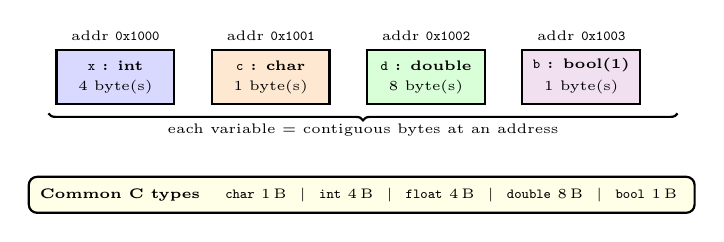
\begin{tikzpicture}[scale=0.68,every node/.style={font=\scriptsize}]
% memory boxes
\foreach \i/\name/\type/\bytes/\col in {0/x/int/4/blue!15,1/c/char/1/orange!18,2/d/double/8/green!15,3/b/bool(1)/1/violet!12} {
  \pgfmathsetmacro{\x}{\i*2.9}
  \draw[thick,fill=\col] (\x,0) rectangle (\x+2.2,1.0);
  \node[font=\tiny\bfseries] at (\x+1.1,0.72) {\texttt{\name} : \type};
  \node[font=\tiny] at (\x+1.1,0.32) {\bytes\ byte(s)};
  \node[font=\tiny,fill=white,inner sep=1pt,rounded corners=1pt] at (\x+1.1,1.28) {addr \texttt{0x100\i}};
}
\draw[decorate,decoration={brace,mirror},thick] (-0.15,-0.18)--(11.6,-0.18) node[midway,below,font=\tiny] {each variable = contiguous bytes at an address};
% type table inset
\node[draw,thick,rounded corners=3pt,fill=yellow!10,align=left,font=\tiny,inner sep=4pt] at (5.7,-1.7) {
  \textbf{Common C types} \quad \texttt{char} 1\,B\ \ $\vert$\ \ \texttt{int} 4\,B\ \ $\vert$\ \ \texttt{float} 4\,B\ \ $\vert$\ \ \texttt{double} 8\,B\ \ $\vert$\ \ \texttt{bool} 1\,B
};
\end{tikzpicture}
\caption{Variables as typed byte-boxes in memory. The type dictates size and interpretation; the address is where the box lives.}
\label{fig:boxes-memory}
\end{figure}

\begin{lstlisting}[language=C]
int     age = 19;           // 4 bytes, signed -2^31 .. 2^31-1
char    grade = 'A';        // 1 byte, single quotes
double  gpa = 4.75;         // 8 bytes, floating point
_Bool   done = 0;           // 0 false, nonzero true (#include <stdbool.h> gives bool)
const int MAX = 100;        // const: cannot be reassigned
\end{lstlisting}
C is \emph{statically typed}: the type is fixed at declaration. Initialise always --- an uninitialised \texttt{int} holds garbage (whatever bits were there before).

Integer promotion and truncation matter: assigning \texttt{300} to a \texttt{char} keeps only the low 8 bits. Use \texttt{sizeof(int)} to query size portably.

\section{Input and Output}
\label{sec:io}
\texttt{printf} formats output; \texttt{scanf} parses input. Both use \emph{format specifiers} that must match the variable type.

\begin{lstlisting}[language=C]
#include <stdio.h>
int main(void){
    int age; double gpa;
    printf("Enter age and GPA: ");
    if (scanf("%d %lf", &age, &gpa) != 2){ // & = address-of (Ch.2)
        printf("Bad input!\n"); return 1;
    }
    printf("Age %d, GPA %.2f\n", age, gpa); // %.2f = 2 decimal places
    return 0;
}
\end{lstlisting}
Common specifiers: \texttt{\%d} int, \texttt{\%c} char, \texttt{\%f} float, \texttt{\%lf} double, \texttt{\%s} string (char array). Always check \texttt{scanf}'s return value: it counts successful conversions.

Buffering note: \texttt{printf} may not appear until newline \texttt{\textbackslash n} or \texttt{fflush(stdout)}.

\section{Control Flow: Branching and Loops}
\label{sec:control}
Programs need decisions and repetition. C provides both with minimal syntax.

\subsection{Branching}
\begin{lstlisting}[language=C]
int score = 82;
if (score >= 80)       printf("A\n");
else if (score >= 70)  printf("B\n");
else                   printf("C\n");

char op = '+';
switch(op){            // switch: jump table on integer/char
    case '+': printf("add\n"); break;
    case '-': printf("sub\n"); break;
    default:  printf("other\n");
}
\end{lstlisting}
\texttt{break} exits the \texttt{switch}; without it execution \emph{falls through}. Braces \texttt{\{\}} group multiple statements.

\subsection{Loops}

\begin{figure}[h]\centering
\begin{tikzpicture}[scale=0.70,every node/.style={font=\scriptsize}]
\node[draw,thick,rounded corners=3pt,fill=green!14,minimum width=2.2cm,minimum height=0.7cm] (init) at (0,0) {\texttt{init: i=0}};
\node[draw,diamond,thick,fill=orange!18,aspect=2.2,inner sep=1pt] (cond) at (3.2,0) {i<n?};
\node[draw,thick,rounded corners=3pt,fill=blue!12,minimum width=2.2cm,minimum height=0.7cm] (body) at (6.5,0) {body};
\node[draw,thick,rounded corners=3pt,fill=violet!12,minimum width=2.0cm,minimum height=0.7cm] (upd) at (6.5,-1.7) {\texttt{i++}};
\node[draw,thick,rounded corners=3pt,fill=gray!15,minimum width=1.6cm,minimum height=0.7cm] (done) at (3.2,-1.7) {done};
\draw[-{Latex},thick,blue!60!black] (init)--(cond);
\draw[-{Latex},thick,blue!60!black] (cond)-- node[above,font=\tiny] {yes} (body);
\draw[-{Latex},thick,blue!60!black] (cond)-- node[right,font=\tiny] {no} (done);
\draw[-{Latex},thick,blue!60!black] (body)--(upd);
\draw[-{Latex},thick,blue!60!black] (upd) -- (3.2,-1.2) -- (cond);
\node[font=\tiny,fill=yellow!12,rounded corners=2pt,inner sep=2pt] at (3.2,1.0) {\texttt{for(init; cond; upd) body} $\equiv$ while loop};
\end{tikzpicture}
\caption{Flow of a \texttt{for} loop: initialise $\to$ test $\to$ body $\to$ update $\to$ test $\dots$ until the condition fails.}
\label{fig:for-flow}
\end{figure}

\begin{lstlisting}[language=C]
for (int i = 0; i < 5; i++)   printf("%d ", i);  // 0 1 2 3 4

int k = 5;
while (k > 0){ printf("%d ", k); k--; }          // 5 4 3 2 1

int n;
do { printf("Enter positive n: "); scanf("%d",&n); } while(n <= 0);
\end{lstlisting}
\texttt{for} is for counted iteration; \texttt{while} for condition-driven; \texttt{do--while} runs at least once. \texttt{break} exits the innermost loop; \texttt{continue} skips to next iteration.

\section{Functions and Scope}
A \emph{function} is a named sub-recipe with parameters and a return value. It enables decomposition and reuse.

\begin{lstlisting}[language=C]
int max2(int a, int b){ return (a > b) ? a : b; } // ternary operator
int main(void){
    int x = max2(3, 7);   // call: arguments copied into parameters
    printf("%d\n", x);    // 7
}
\end{lstlisting}
C passes arguments \emph{by value}: the function receives copies. To let a function modify the caller's variable, pass its address (pointer) --- the subject of Ch.~2. Variables have \emph{block scope}: visible only inside their \texttt{\{\}}.


\section{Operators, Expressions, and Precedence}
An \emph{expression} combines values and operators to produce a new value. C evaluates using precedence (higher binds tighter) and associativity.

\begin{center}\small
\begin{tabular}{cll}
\toprule Prec. & Operator & Associativity\\
\midrule 1 & \texttt{() [] -> .} & left\\
2 & \texttt{! \~{} ++ -- + - * \& (unary)} & right\\
3 & \texttt{* / \%} & left\\
4 & \texttt{+ -} & left\\
5 & \texttt{< <= > >=} & left\\
6 & \texttt{== !=} & left\\
7 & \texttt{\&\&} & left\\
8 & \texttt{||} & left\\
9 & \texttt{?:} & right\\
10& \texttt{= += -=} & right\\
\bottomrule
\end{tabular}
\end{center}
\begin{lstlisting}[language=C]
int a=5,b=2,c=3;
int r = a + b * c;      // 11, not 21: * before +
int s = (a+b)*c;        // 21: parentheses override
int t = a > b && b < c; // 1 (true): relational before logical
// Pitfall: == vs =  (comparison vs assignment)
if(a == 5) printf("yes\n"); // correct
// if(a = 5) always true (assigns 5, yields 5 which is truthy) -- bug!
\end{lstlisting}
Integer division truncates towards zero: \texttt{7/2==3}, \texttt{7\%2==1}. Mixing signed/unsigned promotes to unsigned --- a frequent bug source. When in doubt, parenthesise.

\section{Worked Example: Grading Program}
We combine all ideas into a small program that reads scores and prints a grade, demonstrating I/O, branching, loops, and functions.

\begin{lstlisting}[language=C]
#include <stdio.h>
char grade_of(int score){
    if(score>=80) return 'A';
    if(score>=70) return 'B';
    if(score>=50) return 'C';
    return 'F';
}
int main(void){
    int n; printf("How many scores? ");
    if(scanf("%d",&n)!=1 || n<=0) return 1;
    for(int i=0;i<n;i++){
        int s; printf("Score %d: ", i+1);
        scanf("%d",&s);
        printf(" -> Grade %c\n", grade_of(s));
    }
    return 0;
}
\end{lstlisting}
Trace with input \texttt{2 85 62}: \texttt{n=2}, loop \texttt{i=0} reads 85 $\to$ A, \texttt{i=1} reads 62 $\to$ C. Each function call gets its own frame (Ch.~2).

\section{Chapter Notes}
Kernighan \& Ritchie \emph{The C Programming Language} (2nd ed.) remains the canonical reference. \texttt{gcc -Wall -Wextra -std=c11} enables all warnings --- treat warnings as errors early.

\section{Exercises}
\begin{enumerate}[label=E1.\arabic*, leftmargin=*, itemsep=0.6em]
\item \textbf{Trace.} What does this print? \texttt{int a=5,b=2; printf("\%d \%d \%d",a/b, a\%b, (double)a/b);} Explain each expression.
\item \textbf{scanf pitfalls.} Why does \texttt{scanf("\%d", age)} (without \&) often segfault? What does checking \texttt{scanf}'s return value protect against?
\item \textbf{Loop rewrite.} Rewrite \texttt{for(int i=0;i<n;i++) sum+=i;} as a \texttt{while} loop and as a \texttt{do--while} loop. When do the three forms behave differently?
\item \textbf{Fall-through bug.} Write a \texttt{switch} on \texttt{char grade} that maps \texttt{'A'/'B'/'C'/'D'/'F'} to messages, correctly using \texttt{break}. Show a version where a missing \texttt{break} causes a wrong message.
\item \textbf{Function scope.} Write \texttt{int factorial(int n)} iteratively and recursively. Call both from \texttt{main} and explain why the recursive version needs a base case; what happens without it?
\end{enumerate}
% End of Chapter 1
